% Software Requirements
% CS 461 - CS Senior Capstone
% Fall 2017
% Authors: Connor Christensen, Lily Shellhammer, William Buffum


\documentclass[draftclsnofoot,onecolumn,letterpaper,10pt,compsoc]{IEEEtran}

% Packaging
\usepackage{geometry}
\usepackage{hyperref}
\usepackage{titling}
\usepackage{color}
\usepackage{listings}
\usepackage{cite}
\usepackage{pdfpages}

% Paper type
\geometry{letterpaper, margin=.75in}

% Title page
\title{CS 461 - CS Senior Capstone
	\\Fall 2017
	\\Problem Statement
}


\author{
	Connor I. Christensen \\
	\texttt{chriconn@oregonstate.edu}
	\\
	Lily M. Shellhammer \\
	\texttt{shellhal@oregonstate.edu}
	\\
	William B. Buffum \\
	\texttt{buffumw@oregonstate.edu}
}

\begin{document}

\begin{titlingpage}
    \maketitle
    \begin{abstract}
			Ninkasi Brewing Company is using an outdated brewing operations management system. To update the data management system, the BrewHops team will implement a web application and relational database.
			\\
			\textbf{Keywords:} Brewing, Operations, Management, Ninkasi
    \end{abstract}
		\pagebreak
		\tableofcontents
\end{titlingpage}

\section{Introduction}
	\subsection{Purpose}
    In this document, we outline the requirements for Ninkasi’s brewing operations data management system we will implement. This includes a detailed description of the product created and the technology we will be using to complete the product. This document is intended for a technical audience and will be used primarily by our instructors, Kirsten Winters and Kevin McGrath, and our sponsor, Daniel Sharp.
    
	\subsection{Scope}
    We will develop a web application and relational database model to manage Ninkasi data. We will perform a cost-benefit analysis to recommend hosting system with web service provider versus hosting on Ninkasi servers. Database will store: beer type identifier, batch number, GEN\footnote{Need clarification from Daniel on what this is}, Dry Hop/Adjunct Type\footnote{Need clarification from Daniel on what this is}, hop amount, and data on internal brewing vat (IBV) measurements. IBV data points include: S.G.\footnote{Need clarification from Daniel on what this is}, pH level, Alcohol By Volume (ABV), and beer temperature. Provided interface will allow brewers to manually insert new batch records, update incorrect data, and view existing data. Interface will allow Ninkasi personnel to view data using downloadable .csv files. We will gage adequacy of interface based on 60% approval from Ninkasi personnel, of which Daniel Sharp must approve. The goal of these requirements is to stop paper tracking of information and stop use of Excel as primary data storage.
    \\
    \\
    Stretch goals include: login system and data viewing in browser (no download required).
    \\
    \\
    We are not be responsible for application security, data integrity (during manual entry), or direct control of any brewing process.
    
	\subsection{Definitions, acronyms and abbreviations}
    Data collected by our database will be referred to as “cellaring data”. This means data that has been collected while cellaring beers. Data points include but are not limited to: beer temperature, maturation time, amount of hops and other materials added. 
    
	\subsection{References}
    No references as of 10/27/2017.
	\subsection{Overview}
    In the next sections, this document outlines details on the hardware, software, and user interface requirements for our project. It explains what needs to be done in order to launch our minimum viable product. Security, functionality, and organization are explained in detail.

\section{Description}
	\subsection{Product Perspective}
		\subsubsection{System interfaces}
		\subsubsection{User interfaces}
		\subsubsection{Hardware interfaces}
		\subsubsection{Software interfaces}
		\subsubsection{Communications interfaces}
		\subsubsection{Memory constraints}
		\subsubsection{Site adaptation requirements}
	\subsection{Product functions}
	\subsection{User characteristics}
	\subsection{Constraints}
		\subsubsection{Regulatory policies}
		\subsubsection{Hardware limitations (e.g., signal timing requirements)}
		\subsubsection{Interfaces to other applications}
		\subsubsection{Parallel operation}
		\subsubsection{Audit functions}
		\subsubsection{Control functions}
		\subsubsection{Higher-order language requirements}
		\subsubsection{Signal handshake protocols (e.g., XON-XOFF, ACK-NACK)}
		\subsubsection{Reliability requirements}
		\subsubsection{Criticality of the application}
		\subsubsection{Safety and security considerations.}
	\subsection{Assumptions and dependencies}

\section{Specific requirements}
	\subsection{External interfaces}
	\subsection{Functions}
	\subsection{Performance requirements}
	\subsection{Logical database requirements}
	\subsection{Design constraints}
		\subsubsection{Standards compliance}
	\subsection{Software system attributes}
		\subsubsection{Reliability}
		\subsubsection{Availability}
		\subsubsection{Security}
		\subsubsection{Maintainability}
		\subsubsection{Portability}
	\subsection{Organizing the specific requirements}
		\subsubsection{System mode}
		\subsubsection{User class}
		\subsubsection{Objects}
		\subsubsection{Feature}
		\subsubsection{Stimulus}
		\subsubsection{Response}
		\subsubsection{Functional hierarchy}
	\subsection{Comments}
\section{Appendixes}
\section{Index}

\pagebreak
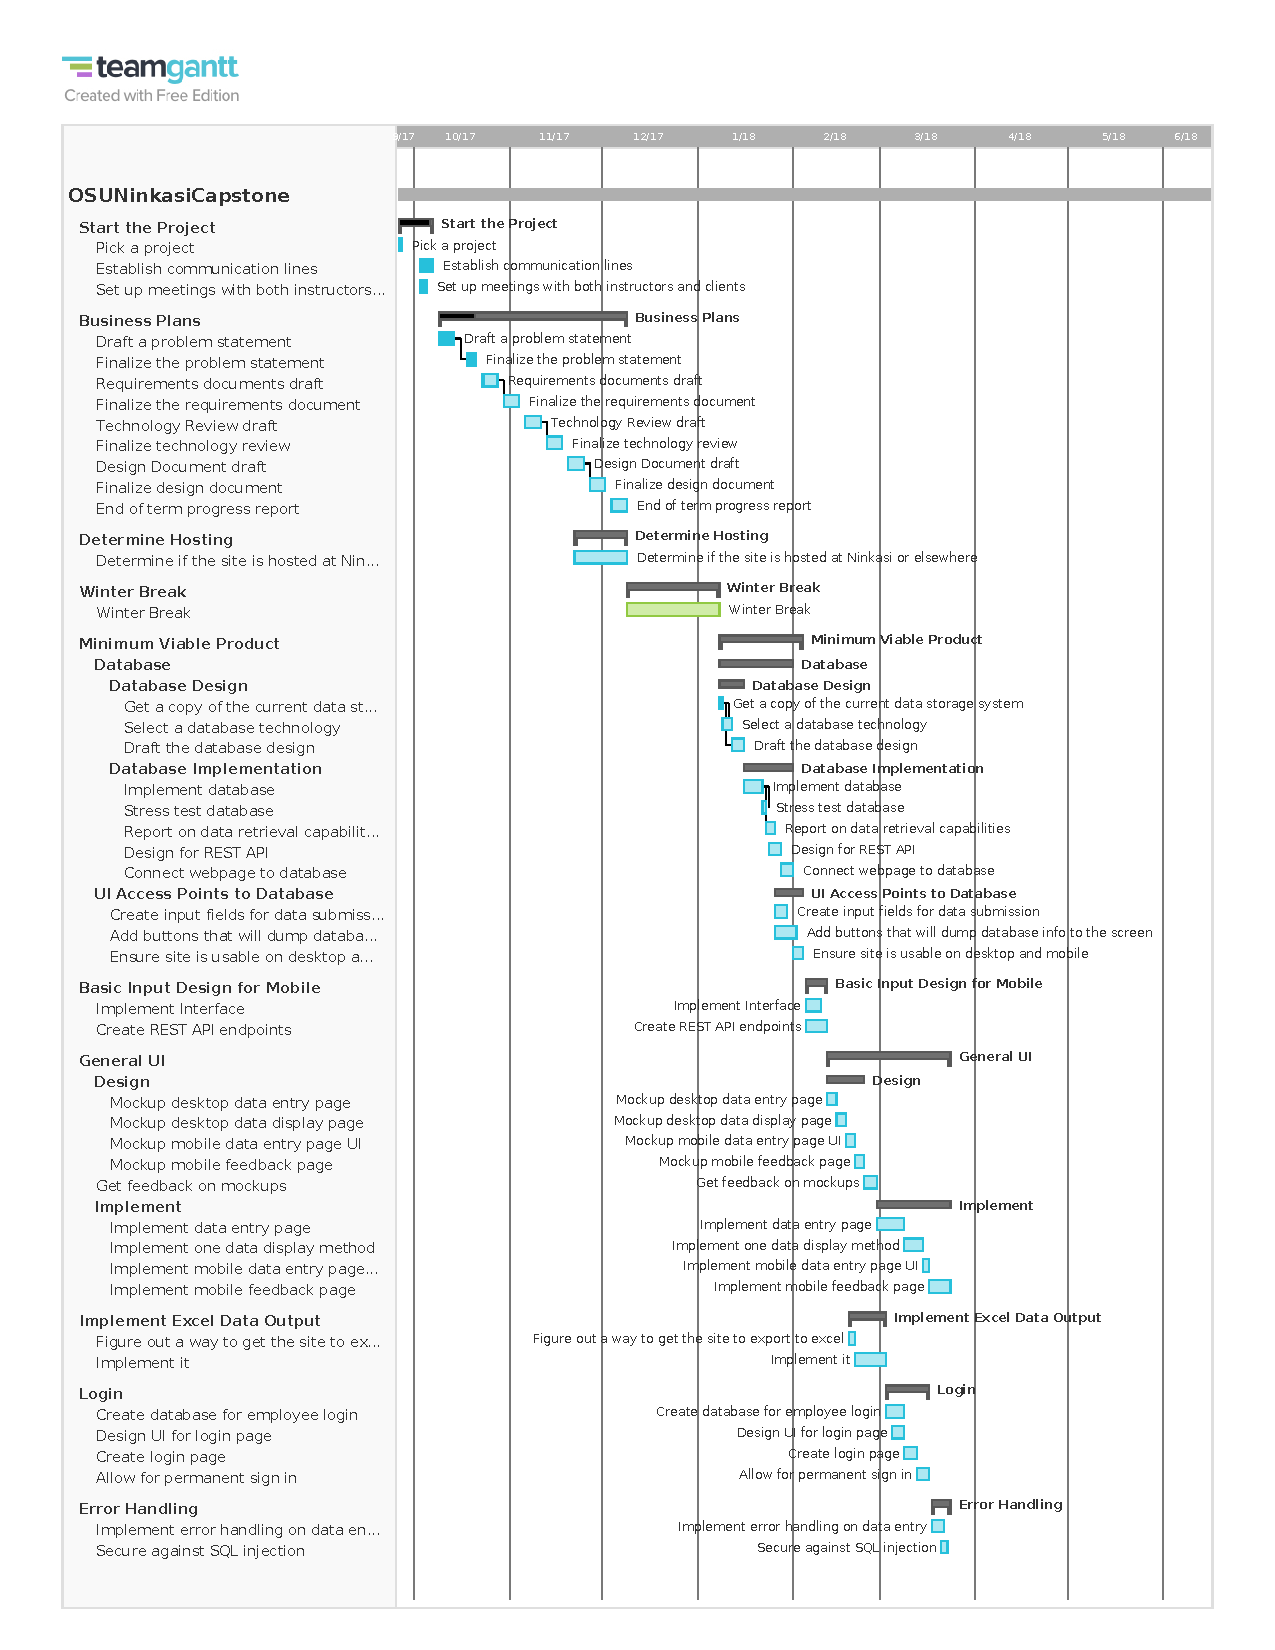
\includepdf[pages=1-2]{OSUNinkasiCapstone.pdf}

\end{document}
